\chapter{FDTD Methods and Analysis Techniques}\label{ch:FDTD}

\begin{flushright}{\it
``Since Newton, mankind has come to realize that the laws of physics\\
are always expressed in the language of differential equations.''\\
- Steven Strogatz\\
\SWcomment[(https://youtu.be/O85OWBJ2ayo?t=44)]} 
\end{flushright}
%
This chapter introduces some important concepts needed to understand the physical models presented later on in this document. 
By means of a simple mass-spring system and the 1D wave equation, the notation (and terminology) used throughout this document will be explained, together with some important analysis techniques. 
Before we dive into the mathematics, let us go over some useful terminology.

\subsubsection{Differential equations}
As mentioned in Chapter \ref{ch:physMod} differential equations are used to describe the motion of dynamic systems. These systems can describe anything from the transverse displacement of a string to the air pressure in an acoustic tube.

A characteristic feature of these equations is that, rather than an absolute value or \textit{state} of a system, the time derivative of its state -- its velocity -- or the second-order time derivative -- its acceleration -- is described. From this, the absolute state of the system can be computed.

This state is usually described by the variable $u$ which is (nearly) always a function of time, i.e., $u=u(t)$. If the system is distributed in space, $u$ also becomes a function of space, i.e., $u = u(x,t)$, or with two spatial dimensions, $u = u(x,y,t)$, etc. Though this work only describes systems of up to two spatial dimensions, one could potentially extend to systems of infinite spatial dimensions evolving over time! 

If $u$ is only a function of time, the differential equation that describes the motion of this system is called an \textit{ordinary differential equation} (ODE). If $u$ is also a function of at least one spatial dimension, the equation of motion is a called a \textit{partial differential equation} (PDE).

The literature uses different types of notation for taking (continuous-time) partial derivatives. Applied to a state variable $u$ these can look like 
%
\begin{equation}\nonumber
    \begin{aligned}
        \frac{\partial^2 u}{\partial t^2} & \quad \text{(classical notation)}\\
        u_{tt}\:\,& \quad \text{(subscript notation)}\\[3pt]
        \ptt u\: & \quad \text{(operator notation)}
    \end{aligned}
\end{equation}
%
all of which mean a second-order derivative with respect to time $t$, i.e., $u$'s acceleration. In this remainder of this document, the operator notation will be used. Often-used partial derivatives and their interpretation \todo{maybe not yet as this is super general still} are shown below

\begin{minipage}[c]{0.49\textwidth}
    \begin{align*}
        \ptt u &\quad \text{(acceleration)}\\
        \pt u &\quad \text{(velocity)}
    \end{align*}
\end{minipage}
\begin{minipage}[c]{0.49\textwidth}
    \begin{align*}
    \pxx u &\quad \text{(curvature)}\\
    \px u &\quad \text{(slope)}
    \end{align*}
\end{minipage}

\textit{Note: difference between 1D, 2D spatial, and 1D, 2D displacement (polarisation). Transverse displacement of 1D wave here }

Now that an equation has been established, how 


\subsubsection{Discretisation using FDTD methods}
Finite-difference time-domain (FDTD) methods essentially subdivide a continuous equation in discrete points in time and space, a process called \textit{discretisation}. Once an ODE or PDE is discretised using these methods it is now called a \textit{Finite-Difference (FD) Scheme}.

We start by defining a discrete \textit{grid} over time and space which we will use to approximate our continuous equations \todo{grid figure}. A system $u = u(x,t)$ defined over time $t$ and one spatial dimension $x$, can be approximated using a \textit{grid function} $u_l^n$. Here, subscript $l$ superscript $n$ describe the spatial and temporal indices respectively and arise from the discretisation of the continuous variables $x$ and $t$ according to $x=lh$ and $t=nk$. The spatial step $h$, also called the \textit{grid spacing} describes the distance (in m) between two neighbouring grid points and the temporal step $k$, or \textit{time step} is the time (in s) between two consecutive temporal indices. The latter can be calculated $k=1/\fs$ for a sample rate $\fs$ (in Hz). In many audio applications $\fs = 44100$ Hz which will be used in this work (unless denoted otherwise).

To summarise
\begin{equation}
    u(x,t) \approx u_l^n \quad \text{with} \quad x=lh \quad \text{and} \quad t = nk
\end{equation}

Now that the state variable has a discrete counterpart, this leaves the derivatives to be discretised. We start by introducing shift operators that can be applied to a grid function and changes its indexing (either spatial or temporal). Forward and backward shifts in time, together with the identity operation (not altering $\uln$) are
% 
\begin{equation}
    e_{t+}\uln = u_l^{n+1},\quad e_{t-}\uln = u_l^{n-1}, \quad \text{and} \quad 1\uln = \uln.
\end{equation}
%
Similarly, forward and backward shifts in space are
%
\begin{equation}
    e_{x+}\uln = u_{l+1}^n,\quad \text{and}\quad e_{x-}\uln = u_{l-1}^n.
\end{equation}
%
These shift operators are rarely used in isolation, though they do appear in energy analysis techniques detailed in Section \ref{sec:energyAnalysis}. The operators do, however, form the basis of commonly used FD operators. The first-order derivative in time can be discretised three different ways. The forward, backward and centred \todo{check centred instead of centered, full document sweep} difference are
%
\begin{subnumcases}{\pt \approx\label{eq:discFirstTime}}
        \dtp &$\!\!\!\!\!\!\!\!\!\!\triangleq \frac{1}{k}\left(e_{t+} - 1\right),$\label{eq:forwardTimeOperator}\\
        \dtm &$\!\!\!\!\!\!\!\!\!\!\triangleq \frac{1}{k}\left(1 - e_{t-}\right),$\label{eq:backwardTimeOperator}\\
        \dtd &$\!\!\!\!\!\!\!\!\!\!\triangleq \frac{1}{2k}\left(e_{t+} - e_{t-}\right),$\label{eq:centredTimeOperator}
\end{subnumcases}
where ``$\triangleq$'' means ``equal to by definition''. These operators can then be applied to grid function $\uln$ to get
\begin{subnumcases}{\pt u \approx\label{eq:discFirstTimeU}}
    \dtp \uln &$\!\!\!\!\!\!\!\!\!\! = \frac{1}{k}\left(u_l^{n+1} - \uln\right),$\label{eq:forwardTimeOperatorU}\\
    \dtm \uln &$\!\!\!\!\!\!\!\!\!\! = \frac{1}{k}\left(\uln - u_l^{n-1}\right),$\label{eq:backwardTimeOperatorU}\\
    \dtd \uln &$\!\!\!\!\!\!\!\!\!\! = \frac{1}{2k}\left(u_l^{n+1} - u_l^{n-1}\right).$\label{eq:centredTimeOperatorU}
\end{subnumcases}
Note that the centred difference has a division by $2k$ as the time difference between $n+1$ and $n-1$ is twice the time step. 

\todo{figure here for interpretation of accuracy of operators}
The same can be done in for a first-order derivative in space, where the forward, backward and centred difference are
\begin{subnumcases}{\px \approx\label{eq:discFirstSpace}}
    \dxp &$\!\!\!\!\!\!\!\!\!\!\triangleq \frac{1}{h}\left(e_{x+} - 1\right),$\label{eq:forwardSpaceOperator}\\
    \dxm &$\!\!\!\!\!\!\!\!\!\!\triangleq \frac{1}{h}\left(1 - e_{x-}\right),$\label{eq:backwardSpaceOperator}\\
    \dxd &$\!\!\!\!\!\!\!\!\!\!\triangleq \frac{1}{2h}\left(e_{x+} - e_{x-}\right),$\label{eq:centredSpaceOperator}
\end{subnumcases}
and when applied to $\uln$ are
\begin{subnumcases}{\px u \approx\label{eq:discFirstSpace}}
    \dxp \uln&$\!\!\!\!\!\!\!\!\!\!= \frac{1}{h}\left(u_{l+1}^n- \uln\right),$\\
    \dxm \uln&$\!\!\!\!\!\!\!\!\!\!= \frac{1}{h}\left(\uln - u_{l-1}^n\right),$\\
    \dxd \uln&$\!\!\!\!\!\!\!\!\!\!= \frac{1}{2h}\left(u_{l+1}^n - u_{l-1}^n\right).$\label{eq:centredSpaceOperatorU}
\end{subnumcases}
Higher order differences can be obtained from first-order difference operators. The second-order difference in time may be approximated using
\begin{equation}\label{eq:discSecondTime}
    \ptt \approx \dtp\dtm = \dtt = \frac{1}{k^2}\left(e_{t+}-2+e_{t-}\right),
\end{equation}
where ``2'' is the identity operator applied twice.  and similarly for the second-order difference in space
\begin{equation}\label{eq:discSecondSpace}
    \pxx \approx \dxp\dxm = \dxx = \frac{1}{h^2}\left(e_{x+}-2+e_{x-}\right).
\end{equation}
More explanation about combining operators can be found in Section \ref{sec:combiningOperators}.

Averaging operators



Operators and derivatives in 2D will be discussed in Chapter \ref{ch:2Dsyst}.
\subsubsection{Accuracy}
Taylor series expansion...
\subsection{Identities}
Extremely useful are

An identity is something that holds true 
\begin{subequations}
    \begin{align}
        \dtt \uln &= \frac{2}{k}\left(\dtd \uln - \dtm \uln\right)\\
        \dtt &
    \end{align}
\end{subequations}
That these identities hold can easily be proven by expanding the operators
\subsubsection{Implementation}
In the following 
\begin{itemize}
    \item Continuous-time
    \item Discrete-time
    \item Implementation (update equation)
\end{itemize}


Something something newton's second law

initial conditions

It is important to note that a discrete FD scheme is an \textit{approximation} to a continuous PDE, not a sampled version of it. This means that the resulting schemes are rarely an exact solution to the original continuous equation.

\section{%Intro to ODEs: 
The Mass-Spring System}
Though a complete physical modelling field on its own (see Chapter \ref{ch:physMod}), mass-spring systems are also sound-generating systems themselves.

\subsubsection{Continuous-time}
The ODE of a simple mass-spring system is defined as
\begin{equation}\label{eq:massSpringPDE}
    \frac{d^2u}{dt^2} = -\omega_0^2u
\end{equation}

\subsubsection{Discrete-time}
The , $u$ is approximated using 
\begin{equation}
    u(t) \approx u^n
\end{equation}
where $t = nk$

\subsubsection{Implementation}


\section{%Intro to PDEs: 
The 1D Wave Equation}
Arguably the most important PDE in the field of physical modelling for sound synthesis is the 1D wave equation. %Consider state variable $u=u(x,t)$
% Note that the $\partial$ symbol is used rather than the $d$ as in \eqref{eq:massSpringPDE} as it


\subsection{Continuous-time}
The state of the system $u=u(x,t)$ meaning that is on top of being defined in time $t$ it is distributed over space $x$. The 1D wave equation is defined as follows
\begin{equation}\label{eq:1DwavePDE}
    \ptt u = c^2 \pxx u,
\end{equation}
where $c$ is the wave speed (in m/s). The state variable $u$ can be used to describe transverse vibration in an ideal string, longitudinal vibration in an ideal bar and pressure in an acoustic tube. Although the behaviour of this equation alone does not appear in the real world, as no physical system is ideal, it is extremely useful as a test case and a basis for more complicated models. Here, it will be used to introduce various concepts and analysis techniques in the field of FDTD methods.

\subsubsection{Intuition}
Although the 1D wave equation often appears in the literature, an intuition or interpretation of why it works the way it does is hard to find. In the following, $u$ describes the transverse displacement of an ideal string.

Going back to Newton's second law

The acceleration of $u = u(x,t)$ at location $x$ is determined by the second-order spatial derivative of $u$ at that same location (scaled by a constant $c^2$). In the case that $u$ describes the transverse displacement of an ideal string, this second-order derivative denotes the \textit{curvature} of this string. As $c^2$ is always positive, the sign (or direction) of the acceleration is fully determined by the sign of the curvature. In other words, a `positive' curvature at location $x$ along the ideal string yields a `positive' or upwards acceleration at that same location. 

What a `positive' or `negative' curvature implies is more easily seen when we take a simple function describing a parabola, $y(x) = x^2$, and take its second derivative to get $y''(x) = 2$. The answer is a positive number which means that $y$ has a positive curvature. 

So, what does this mean for the 1D wave equation? As a positive curvature implies a positive or upwards acceleration as per Eq. \eqref{eq:1DwavePDE}, $u$ with a positive curvature at a location $x$ will start to move upwards and vice versa. Of course, the state of a physical system such as $u$ will rarely have a perfect parabolic shape, but the argument still applies. 

\begin{figure}[h]
    \centering
    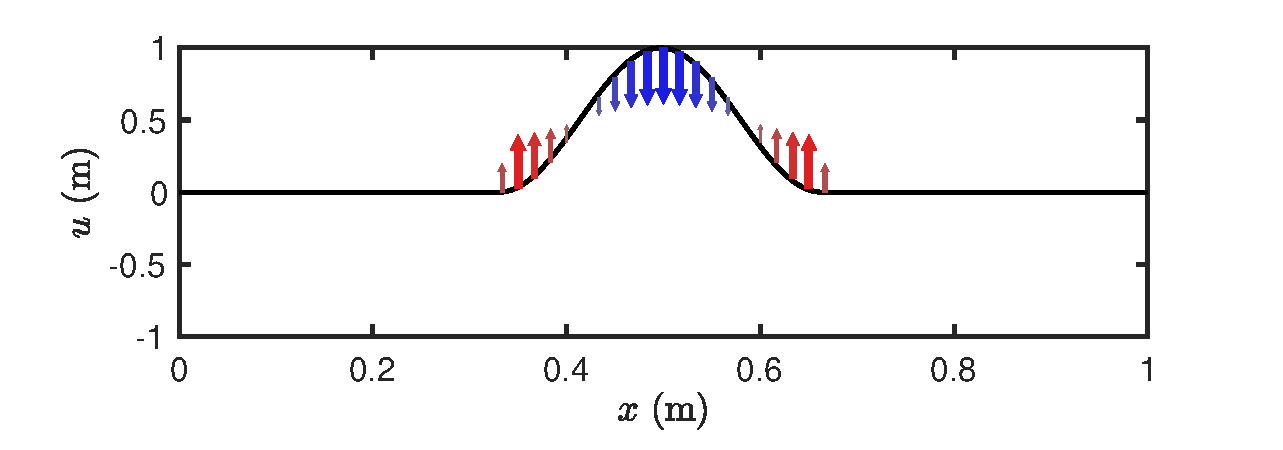
\includegraphics[width=\textwidth]{figures/resonators/curvature.eps}
    \caption{\label{fig:curvature} The forces acting on the 1D wave equation initialised with a raised cosine at $x = 0.5$. Arrows indicate the direction and magnitude of the force.}
\end{figure}

\subsubsection{Boundary Conditions}
When a system is distributed in space, 

For analysis purposes, an infinite domain may be adopted, but for implementation, a finite domain needs to be established. 

Consider a system of length $L$ (in m) $x\in \D$ ($x$ is an element in $\D$) where domain $\D = [0, L]$
Two alternatives are

\begin{subequations}\label{eq:boundaryCond1DWave}
    \begin{align}
        u(0, t) = u(L, t) &= 0\quad \text{(Dirichlet, fixed)},\label{eq:contDirichlet}\\
        \px u(0, t) = \px u(L, t) &= 0\quad \text{(Neumann, free)},\label{eq:contNeumann}
    \end{align}
\end{subequations}

\subsection{Discrete-time}
The most straightforward discretisation of Eq. \eqref{eq:1DwavePDE} is the following FD scheme
\begin{equation}\label{eq:1DwaveFDS}
    \dtt \uln = c^2 \dxx \uln.
\end{equation}
Other schemes exist (such as implicit)
\subsubsection{Stability}
The parameters that define \eqref{eq:1DwaveFDS} are linked through a stability condition. The famous Courant-Friedrichs-Lewy or \textit{CFL condition} is defined as \cite{courant} 
\begin{equation}\label{eq:CFL}
    \lambda \leq 1 \quad \text{where} \quad \lambda = \frac{ck}{h}
\end{equation}
where
\begin{equation}\label{eq:courantNumber}
    \lambda = \frac{ck}{h}
\end{equation}
is referred to as the \textit{Courant number}.

Regarding implementation, as the time step $k$ is based on the sample rate and thus usually fixed and $c$ is a user-defined wavespeed, it is useful to rewrite Eq. \eqref{eq:CFL} to be in terms of the grid spacing $h$:
\begin{equation}
    h \geq ck.
\end{equation}

\subsubsection{Implementation}
\begin{equation}\label{eq:1DwaveFDS}
    u_l^{n+1} = 2 \uln - u_l^{n-1} + \lambda^2 \left(u_{l+1}^n - 2 \uln + u_{l-1}^n\right)
\end{equation}

If $\lambda = 1$, \eqref{eq:1DwaveFDS} is an exact solution to Eq. \eqref{eq:1DwavePDE}. This is no


\subsubsection{Matrix form}
\subsection{Operators in Matrix Form}
Finite-difference operators, such as $\delta_{x+}$,  $\delta_{x-}$ and $\delta_{x\cdot}$ can be written in matrix form:
\begin{gather*}\small
    \mathbf{D}_{x+} = \frac{1}{h}\begin{bmatrix}
        \ddots &\ddots & & & \mathbf{0}&\\
         & -1 & 1 & & & \\
        & & -1 & 1 & & \\
        & & & -1 & 1 & \\
        & & & & -1 & \ddots\\
        &\mathbf{0} & & & & \ddots \\
    \end{bmatrix}
    \quad
    \mathbf{D}_{x-} = \frac{1}{h}\begin{bmatrix}
        \ddots & & & & \mathbf{0}&\\
        \ddots & 1 & & & & \\
        & -1 & 1 & & & \\
        & & -1 & 1 & & \\
        & & & -1 & 1 & \\
        &\mathbf{0} & & & \ddots & \ddots \\
    \end{bmatrix}\\
    \\
    \mathbf{D}_{x\cdot} = \frac{1}{2h}\begin{bmatrix}\small
        \ddots &\ddots & & & \mathbf{0}&\\
        \ddots & 0 & 1 & & & \\
        & -1 & 0 & 1 & & \\
        & & -1 & 0 & 1 & \\
        & & & -1 & 0 & \ddots \\
        &\mathbf{0} & & & \ddots & \ddots \\
    \end{bmatrix}\\
\end{gather*}
The matrices $\mathbf{D}_{x+}$ and $\mathbf{D}_{x-}$ can be multiplied to get $\Dxx$:
\begin{equation}\small
    \Dxx = \mathbf{D}_{x+}\mathbf{D}_{x-} = \frac{1}{h^2}\begin{bmatrix}
        \ddots &\ddots & & & \mathbf{0}&\\
        \ddots & -2 & 1 & & & \\
        & 1 & -2 & 1 & & \\
        & & 1 & -2 & 1 & \\
        & & & 1 & -2 & \ddots \\
        &\mathbf{0} & & & \ddots & \ddots \\
    \end{bmatrix}
\end{equation}
and two $\Dxx$'s to get
\begin{equation}
    \Dxx\Dxx = \mathbf{D}_{xxxx} = \frac{1}{h^4}\begin{bmatrix}
        5& -4 & 1 & & & \mathbf{0}& \\
        -4 & 6 &\ddots &\ddots & & & \\
        1& \ddots & \ddots & -4 & 1 & & \\
        & \ddots& -4 & 6 & -4 & \ddots& \\
        & & 1 & -4 & \ddots & \ddots &1 \\
        & & & \ddots & \ddots & 6 & -4 \\
        & \mathbf{0} & & & 1& -4 & 5 \\
    \end{bmatrix}
\end{equation}
which is used for a stiff string with a simply supported boundary condition.

Averaging operators $\mu_{x+}$, $\mu_{x-}$ and $\mu{x\cdot}$ are defined in a similar way:

\begin{gather*}
    \mathbf{M}_{x+} = \frac{1}{2}\begin{bmatrix}
        \ddots &\ddots & & & \mathbf{0}&\\
         & 1 & 1 & & & \\
        & & 1 & 1 & & \\
        & & & 1 & 1 & \\
        & & & & 1 & \ddots\\
        &\mathbf{0} & & & & \ddots \\
    \end{bmatrix}
    \qquad
    \mathbf{M}_{x-} = \frac{1}{2}\begin{bmatrix}
        \ddots & & & & \mathbf{0}&\\
        \ddots & 1 & & & & \\
        & 1 & 1 & & & \\
        & & 1 & 1 & & \\
        & & & 1 & 1 & \\
        &\mathbf{0} & & & \ddots & \ddots \\
    \end{bmatrix}\\
    \\
    \mathbf{M}_{x\cdot} = \frac{1}{2}\begin{bmatrix}
        \ddots &\ddots & & & \mathbf{0}&\\
        \ddots & 0 & 1 & & & \\
        & 1 & 0 & 1 & & \\
        & & 1 & 0 & 1 & \\
        & & & 1 & 0 & \ddots \\
        &\mathbf{0} & & & \ddots & \ddots \\
    \end{bmatrix}\\
\end{gather*}

Note the multiplication by $1/2$ rather than $1/h$ (or $1/2h$) for all operators.


Only spatial operators are written in this matrix form and then applied to state vectors at different time steps ($n+1$, $n$ and $n-1$), examples of which can be found below.

\subsubsection{Output sound}
After the system is excited (see \ref{part:exciters}), one can listen to the output


\section{Energy Analysis}\label{sec:energyAnalysis}
Debugging physical models.

\subsection{Mathematical tools}
\subsubsection{Continuous-time}
For two functions $f(x)$ and $g(x)$ and $x\in\D$ their $l_2$ inner product along with the $l_2$ norm is defined as
\begin{equation}\label{eq:contInnerProd}
    \langle f, g\rangle_\D \int_\D fg dx \quad \text{and} \quad \lVert f \rVert_\D = \sqrt{\langle f, f \rangle_\D}
\end{equation}


\subsubsection{Discrete-time}
Inner product of any time series $f^n$ and $g^n$ and the discrete counterpart to \eqref{eq:contInnerProd} is
\begin{equation}\label{eq:discInnerProd}
    \langle f^n, g^n \rangle_\D = \sum_{l\in\D} h f_l^n g_l^n
\end{equation}
where the multiplication by $h$ is the discrete counterpart of $dx$ the continuous definition. 

\section{von Neumann Analysis}\label{sec:stabilityAnalysis}
Much literature gives the stability condition using an ``it can be shown that'' argument. Here, I would like to take the opportunity to 

Finding stability conditions for models

Sin identity:
\begin{equation}\label{eq:sinIdentity}
    \sin(x) = \frac{e^{jx} - e^{-jx}}{2j}\quad \Longrightarrow \quad \sin^2(x) = \frac{e^{j2x} - 2e^{jx-jx}+ e^{-j2x}}{-4} = \frac{e^{j2x} + e^{-j2x}}{-4} + \frac{1}{2}.
\end{equation}
Cos identity:
\begin{equation}\label{eq:cosIdentity}
    \cos(x) = \frac{e^{jx} + e^{-jx}}{2}\quad \Longrightarrow \quad \cos^2(x) = \frac{e^{j2x} + 2e^{jx-jx}+ e^{-j2x}}{4} = \frac{e^{j2x} + e^{-j2x}}{4} + \frac{1}{2}.
\end{equation}

\section{Modal Analysis}\label{sec:modalAnalysis}
This section will show how to obtain the modes for an FD scheme implementing the 1D wave equation as done in Section . We start with Eq. (6.34) (using $c$ instead of $\gamma$)
\begin{equation}
    \delta_{tt}u = c^2\delta_{xx}u,
\end{equation}
which can be written in matrix form as
\begin{equation}\label{eq:matrixForm1D}
    \frac{1}{k^2}\left(\u^{n+1}-2\u^n+\u^{n-1}\right) = c^2 \Dxx\u
\end{equation}
Following \cite{theBible} we assume a solution of the form $\u = \boldsymbol{\phi}z^n$. Substituting this into Eq. \eqref{eq:matrixForm1D} yields the characteristic equation
\begin{equation}
    (z - 2 + z^{-1})\boldsymbol{\phi} = c^2k^2\Dxx \boldsymbol{\phi}.
\end{equation}
This is an eigenvalue problem where the $p$'th solution is defined as 
\begin{gather}
    z_p-2+z_p^{-1} = c^2k^2\text{eig}_p(\Dxx)\nonumber\\
    z_p+(-2-c^2k^2\text{eig}_p(\Dxx))+z_p^{-1}=0
\end{gather}
where $\text{eig}_p(\cdot)$ denoting the $p$th eigenvalue of `$\cdot$'. \SWcomment[If the CFL condition for the scheme is satisfied, the roots will lie on the unit circle.] Furthermore we can substitute a test solution $z_p=e^{j\omega_pk}$ solve for the eigenfrequencies:
\begin{align*}
    e^{j\omega_pk}+e^{-j\omega_pk}-2-c^2k^2\text{eig}_p(\Dxx)&=0\\
    \frac{e^{j\omega_pk}+e^{-j\omega_pk}}{-4}+\frac{1}{2}+\frac{c^2k^2}{4}\text{eig}_p(\Dxx)&=0
\end{align*}
Then using Eq. \eqref{eq:sinIdentity} we get
\begin{align}
    \sin^2(\omega_pk/2)+c^2k^2\text{eig}_p(\Dxx)&=0\nonumber\\
    \sin(\omega_pk/2)&=c k\sqrt{-\text{eig}_p(\Dxx)}\nonumber\\
    \omega_p &= \frac{2}{k}\sin^{-1}\left(c k\sqrt{-\text{eig}_p(\Dxx)}\right)
\end{align}
which is Eq. (6.53) in \cite{theBible}.

\section{Dispersion analysis}\label{sec:dispersionAnalysis}
